\subsection{Initial Tasks}
    \begin{task}[label=task:setup]{Set up the directory structure for the workshop.}
    Create directories for:
        \begin{enumerate}[label=(\alph*)]
            \item Structure files
            \item Docking simulations
            \item \gls{acr:md} simulations
            \item Free energy calculations
        \end{enumerate}
    \end{task}

    \paragraph{}
    Firstly, whenever starting any new project, a working directory needs to be created. This can be done either using the \gls{acr:cli} in a terminal using the \enquote{\texttt{mkdir}} command, or using a \gls{acr:gui} file manager. Commands to do this can be found in the cheat codes \cref{cmd:task1}.

\begin{bashoutput}[label=listing:folders]{Folder structure as shown by the \texttt{tree} command.}
    MD_Workshop
    ├── Structures
    ├── Docking
    ├── Dynamics
    └── Free_Energy
\end{bashoutput}
    
    \begin{task}[label=task:Structures]{Obtaining the structure files.}
    \begin{enumerate}[label=(\alph*)]
        \item Obtain the protein crystal structure
        \begin{enumerate}[label=(\roman*)]
            \item Visit the protein database website
            \item Find the protein using code 1n23
            \item Download the crystal structure
        \end{enumerate}
        \item Save the ligand coordinates files located in the workshop files
        \item Split the complex crystal structure into the protein and ligand
    \end{enumerate}
  \end{task}

  \paragraph{}
  There are a few places where you can find and store crystal structure coordinates, however, the main two that are used are \href{https://www.rcsb.org/}{rscb} and \href{https://www.uniprot.org/}{uniprot}. These websites are powerful tools and often group multiple versions of the same protein. Most proteins are published on the rscb database however for unresolved crystal structures, uniprot sometimes also contains the alphafold\cite{Varadi2022AlphaFoldModels} homology model structure. 

  \paragraph{}
  Although we will not be covering the theory or methods of homology modelling in this workshop, being aware of the technique could potentially be useful when working with an unresolved protein structure. The method allows for an approximate structure to be generated using similar proteins as templates. A homology modelling program with growing popularity is the \href{https://www.deepmind.com/research/highlighted-research/alphafold}{alphafold}\cite{Varadi2022AlphaFoldModels} program which uses artificial intelligence to estimate a crystal structure from a FASTA sequence.

  \paragraph{}
  To start this workshop, you will need to visit the rscb website and download the \enquote{pdb} file for the (+)-Bornyl diphosphate synthase which can be found using the code 1N23.  If you google the protein code, it usually comes up as one of the first options. If you have any problems with this then use the commands found in the cheat codes \cref{cmd:task2}. Although there are multiple versions of this protein, we want the structure that has the diphosphate bound separately to the ligand so that we can dock a terpene ligand into the active site.

  \paragraph{}
  You can visualise this protein using \texttt{VMD} to check that the protein is correct (Command \ref{cmd:vmd}). When you open the structure it will likely be in the \enquote{lines} representation, meaning you will struggle to see the protein backbone. It is recommended to change this representation by going into the \enquote{Graphics} menu and selecting \enquote{Representations} (Figure \ref{fig:Repres}). From the new window created, then change the drawing method from \enquote{Lines} to \enquote{NewCartoon} to see the protein backbone structure (Figure \ref{fig:NewCartoon}).
    
    \begin{bashcmd}[label=cmd:vmd]{How to open the structure in VMD}
    vmd 1N23.pdb
    \end{bashcmd}

    \begin{figure}[H]
        \centering
        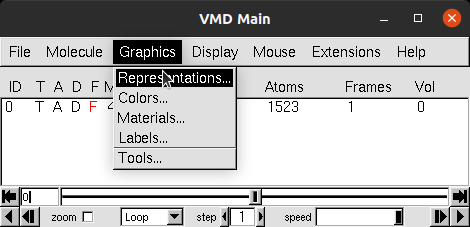
\includegraphics[width=0.7\textwidth]{Graphics/ScreenShots/Representations.png}
        \caption{How to access the representations panel in VMD.}
        \label{fig:Repres}
    \end{figure}

    \begin{figure}[H]
        \centering
        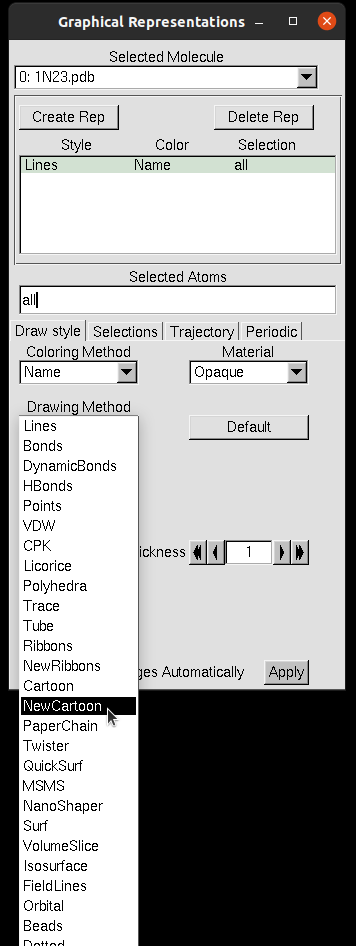
\includegraphics[height=0.7\textheight]{Graphics/ScreenShots/NewCartoonpng.png}
        \caption{How to change the drawing method in VMD.}
        \label{fig:NewCartoon}
    \end{figure}

    \paragraph{}
        Once the protein is correctly visualised, it is often useful to also be able to see the ligand in a \enquote{ball and stick} like representation (known as \enquote{CPK} in VMD). To do this, you first need to know the residue name for the ligand (2BN in this case). You then go back into the graphical representations window and add a new representation using the \enquote{Create Rep} button (Figure \ref{fig:NewRep}). From there you change the selected atoms from \enquote{all} to \enquote{resname 2BN} (Figure \ref{fig:SelectedAtoms}). Finally, you can then change the drawing method to \enquote{CPK} to see the ligand as a ball and stick (Figure \ref{fig:CPK}). The end result should look like Figure \ref{fig:FinalRender}.

    \begin{figure}[H]
        \centering
        \begin{minipage}{0.5\textwidth}
            \centering
            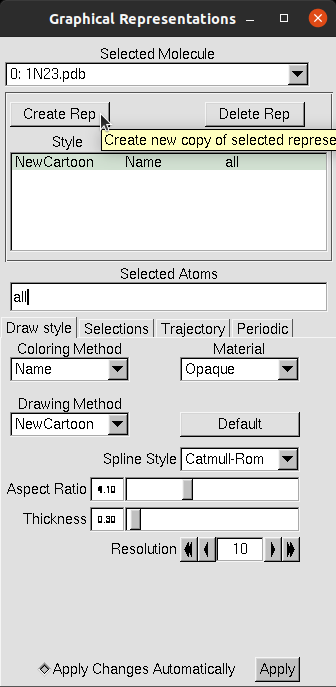
\includegraphics[height=0.4\textheight]{Graphics/ScreenShots/NewRep.png}
            \captionof{figure}{How to create a new \\ representation in VMD.}
            \label{fig:NewRep}
        \end{minipage}%
        \begin{minipage}{0.5\textwidth}
            \centering
            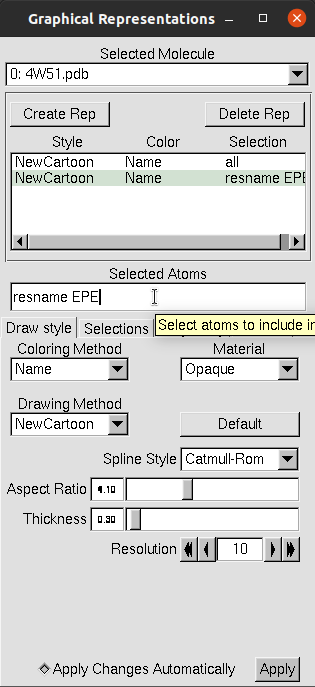
\includegraphics[height=0.4\textheight]{Graphics/ScreenShots/SelectedAtoms.png}
            \captionof{figure}{Changing the selected atoms \\ to the 2BN ligand.}
            \label{fig:SelectedAtoms}
        \end{minipage}
    \end{figure}

    \begin{figure}[H]
        \centering
        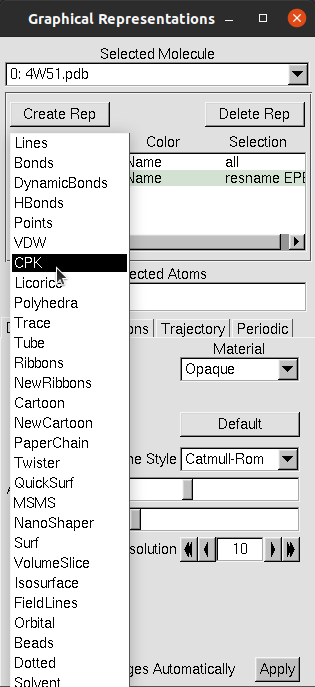
\includegraphics[height=0.4\textheight]{Graphics/ScreenShots/CPK.png}
        \caption{Changing the ligand to the \enquote{CPK} representation.}
        \label{fig:CPK}
    \end{figure}

    \begin{figure}[H]
        \centering
        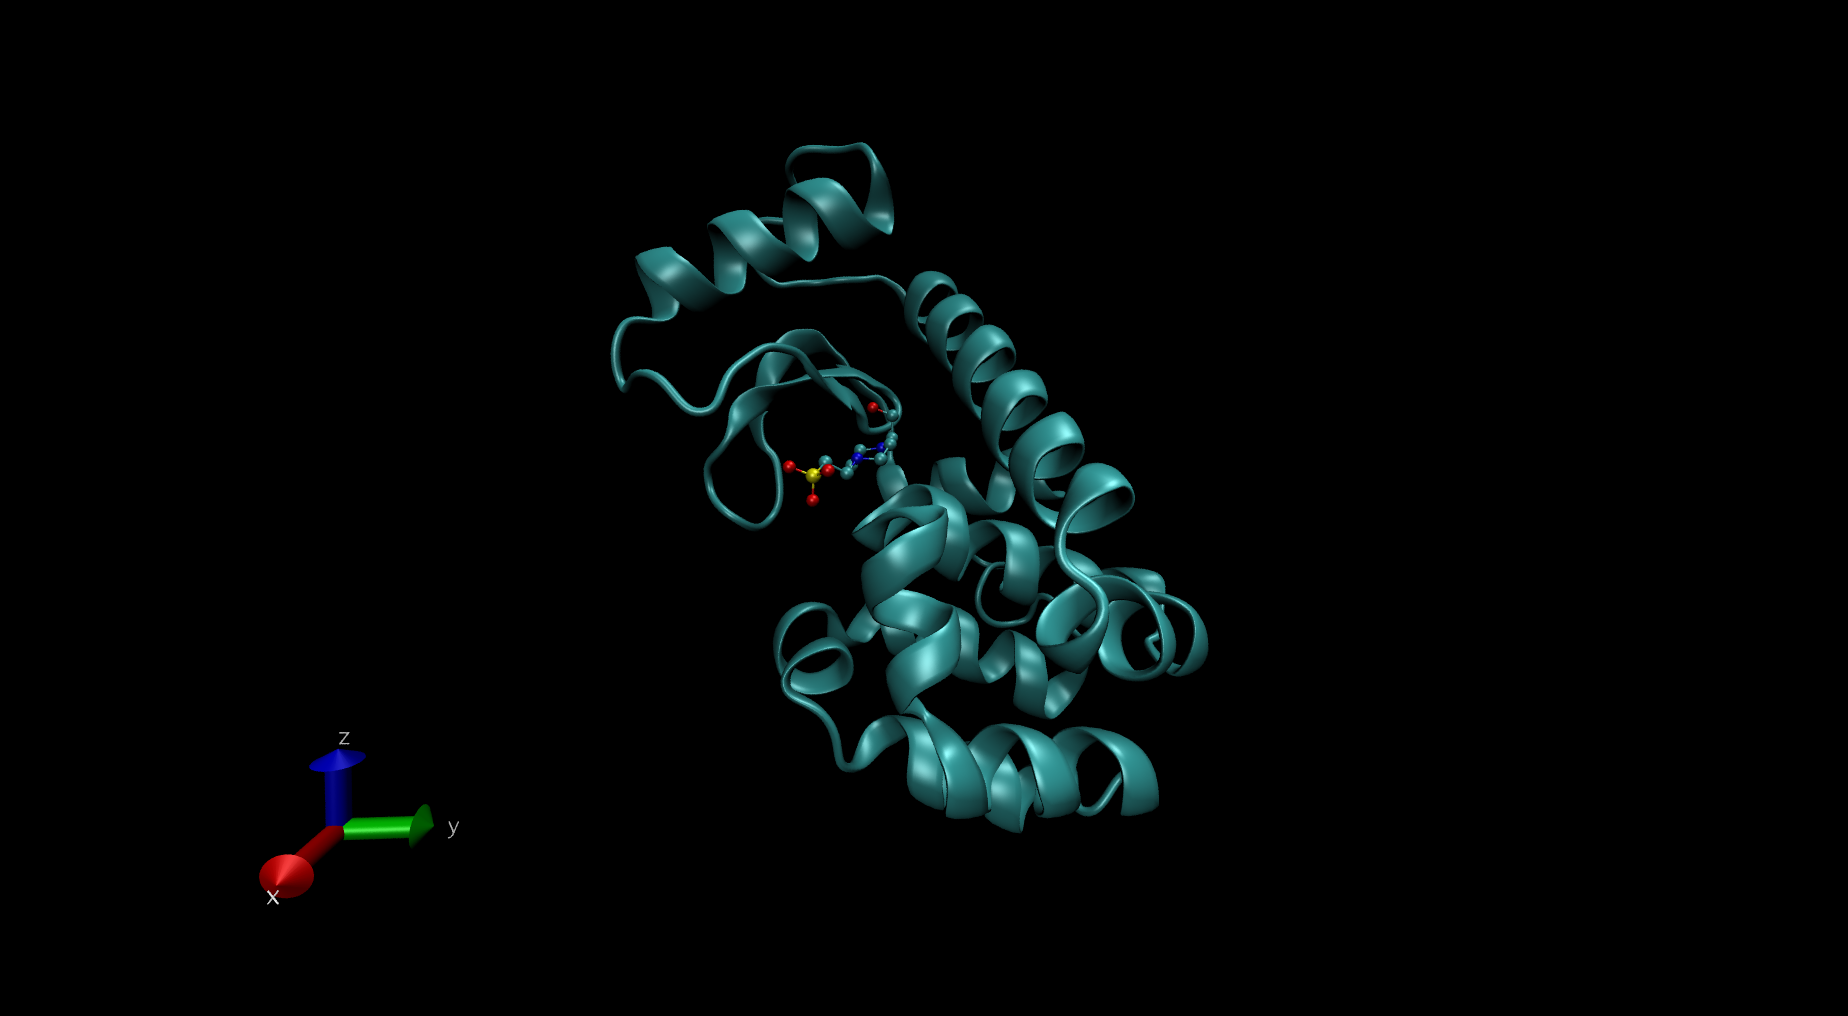
\includegraphics[width=.9\textwidth]{Graphics/ScreenShots/CartoonRender.png}
        \caption{The final render state for visualising the protein and ligand.}
        \label{fig:FinalRender}
    \end{figure}

    \paragraph{}
        Finally, once you have checked that the protein is correct using VMD, you can split the complex pdb \enquote{1N23} into its corresponding protein and ligand. You will notice when visualising the structure that it is a dimer complex and so we also want to remove one of the identical protein chains for simplicity. You can do this simply using the \texttt{grep} commands in \cref{cmd:grep}.  Finally, check that the files are correct (you will have to manually remove some of the water molecules from the \enquote{B} chain in \texttt{vim}) and copy the \enquote{2BN.pdb} and \enquote{1n23\textunderscore monomer\textunderscore NoLig.pdb} files into the Docking directory. This can be done using the \enquote{\texttt{cp}} command in the Linux terminal. 

    \begin{bashcmd}[label=cmd:grep]{How to split the complex crystal structure}
    grep -v " B " > 1n23_monomer.pdb
    grep "2BN" 1N23_monomer.pdb > 2BN.pdb
    grep -v "2BN" 1N23_monomer.pdb > 1n23_monomer_NoLig.pdb        
    \end{bashcmd}

    \paragraph{}
        The coordinates of the ligand that we will be simulating during the workshop can be found, along with any other files required can be found on the \href{https://github.com/pcyra2/MD_workshop/tree/main/Files}{GitHub repo} for the workshop. The exact path to the Ligand file is \href{https://raw.githubusercontent.com/pcyra2/MD_workshop/main/Files/Structures/LIG.mol2}{https://raw.githubusercontent.com/pcyra2/MD\textunderscore workshop/main/Files/Structures/LIG.mol2} and can be downloaded from the terminal using the command \texttt{wget}.

    \begin{bashcmd}[label=cmd:wget]{Command to download the ligand structure file.}
        wget https://raw.githubusercontent.com/pcyra2/MD_workshop/main/Files /Structures/LIG.mol2
    \end{bashcmd}
    